\chapter{Validation You Can Trust}\label{ch:validation}

\section{Introduction}\label{sec:val-why}
\epigraph{The first principle is that you must not fool yourself---and you are the easiest person
to fool.}{Richard Feynman, \emph{Cargo Cult Science} \citeyearpar{feynman1974}}

The public leaderboard may seem the obvious way to judge an idea, but it is a poor instrument for
day-to-day decisions. It accepts only five submissions a day. It scores only about half of the 180
test photographs, so its values are noisy. And it displays scores to two decimal places, so a model
that scores 0.405 and one that scores 0.414 both appear as 0.41. At one point we had four
quite different models whose validation scores spanned 0.013, and all four appeared on the
leaderboard as 0.36. Worse, a team that submits many variants and keeps whichever scores best
gradually fits the public half of the test set, which is a form of overfitting to a reused
holdout~\citep{dwork2015,blum2015}. Decisions must therefore be made on a \keyterm{validation split}: a set of
training photographs that we set aside and score locally, with the exact metric, as often as we
like.

This chapter is about making that split trustworthy, and about the many ways in which a validation
number can mislead. Section~\ref{sec:val-split} shows why the split must be made by photograph,
and Section~\ref{sec:val-time} discusses a subtler leak caused by the persistence of filaments over
time. Section~\ref{sec:val-transfer} measures how well validation scores predict the leaderboard.
Section~\ref{sec:val-oracles} introduces oracles, which measure the best result that an idea could
achieve before we spend effort building it, and Section~\ref{sec:val-traps} collects the
ways in which we misled ourselves with validation numbers during the project.

\section{Splitting by photograph}\label{sec:val-split}
The most obvious split, in which we shuffle the \AllRecords{} annotation records and hold out 15\%
of them, is wrong. A photograph labelled by three annotators appears as three records, and a random
split of the records would put some of them in the training set and others in the validation set.
The model would then be validated on photographs it had already seen during training, and its
validation score would be too high for a reason that has nothing to do with generalisation. Such
\keyterm{leakage} of information from the training data into the evaluation is a well-known fault
in applied machine learning~\citep{kaufman2012}.
Figure~\ref{fig:val-split} illustrates the difference.

\begin{figure}[t]
\centering
\begin{tikzpicture}[
  photo/.style={draw=inkmuted, fill=white, minimum width=0.62cm, minimum height=0.62cm, line width=0.6pt},
  rec/.style={circle, minimum size=0.2cm, inner sep=0pt, fill=#1},
  lab/.style={font=\sffamily\scriptsize, text=inksecondary}]
  % left: split by record
  \node[title] at (1.9,1.1) {split by record (leaks)};
  \foreach \i in {0,...,4} \node[photo] (a\i) at (\i*0.8,0) {};
  \foreach \i/\c in {0/vizblue,1/vizblue,2/vizorange,3/vizblue,4/vizorange}
    \node[rec=\c] at ($(a\i)+(-0.15,0.12)$) {};
  \foreach \i/\c in {0/vizorange,2/vizblue,3/vizblue}
    \node[rec=\c] at ($(a\i)+(0.15,0.12)$) {};
  \foreach \i/\c in {0/vizblue,3/vizorange}
    \node[rec=\c] at ($(a\i)+(0,-0.15)$) {};
  \node[lab, align=center] at (1.9,-0.85) {one photograph can feed\\ both training and validation};
  % right: split by photograph
  \begin{scope}[xshift=5.4cm]
    \node[title] at (1.9,1.1) {split by photograph (canonical)};
    \foreach \i in {0,...,4} \node[photo] (b\i) at (\i*0.8,0) {};
    \foreach \i/\c in {0/vizblue,1/vizblue,2/vizorange,3/vizblue,4/vizorange}
      \node[rec=\c] at ($(b\i)+(-0.15,0.12)$) {};
    \foreach \i/\c in {0/vizblue,2/vizorange,3/vizblue}
      \node[rec=\c] at ($(b\i)+(0.15,0.12)$) {};
    \foreach \i/\c in {0/vizblue,3/vizblue}
      \node[rec=\c] at ($(b\i)+(0,-0.15)$) {};
    \node[lab, align=center] at (1.9,-0.85) {every record follows\\ its photograph};
  \end{scope}
  \node[rec=vizblue] at (3.5,-1.65) {}; \node[lab, anchor=west] at (3.62,-1.65) {training record};
  \node[rec=vizorange] at (6.1,-1.65) {}; \node[lab, anchor=west] at (6.22,-1.65) {validation record};
\end{tikzpicture}
\caption{Squares are photographs and dots are their annotation records. Splitting the records at
random (left) puts records of one photograph on both sides of the split. Our canonical split
(right) assigns whole photographs. \drawnin{book/chapters/ch05\_validation.tex}}
\label{fig:val-split}
\end{figure}

Our canonical split, implemented in \file{shared/data\_split.py} and shown in
Listing~\ref{lst:val-split}, therefore assigns whole photographs to one side or the other. It also
\keyterm{stratifies} by GONG station, which means that it splits the photographs of each station
separately, so that both sides see the same mix of image quality. Finally, it uses a fixed random
seed, 2026, so that every experiment on every machine uses the same split. Changing the seed would
silently make every past comparison meaningless, so we treat it as a constant for the life of the
project.

\begin{lstlisting}[caption={The canonical split. From \file{shared/data\_split.py:make\_split}.},label=lst:val-split]
SPLIT_SEED = 2026   # fixed for the life of the project

def make_split(annotation_path, val_fraction=0.15, seed=SPLIT_SEED):
    stem_to_ids, _ = load_records(annotation_path)       # photograph -> its records
    by_site = defaultdict(list)
    for stem in sorted(stem_to_ids):
        by_site[instrument_of(stem)].append(stem)        # stratify by GONG station
    rng = np.random.default_rng(seed)
    train_stems, val_stems = [], []
    for site in sorted(by_site):
        stems = by_site[site]
        rng.shuffle(stems)
        n_val = max(1, round(len(stems) * val_fraction))
        val_stems.extend(stems[:n_val]); train_stems.extend(stems[n_val:])
    return Split(train_stems=sorted(train_stems), val_stems=sorted(val_stems),
                 train_image_ids=[i for s in sorted(train_stems) for i in stem_to_ids[s]],
                 val_image_ids=[i for s in sorted(val_stems) for i in stem_to_ids[s]])
\end{lstlisting}

The result is a training set of \TrainPhotos{} photographs with \TrainRecords{} records and
\TrainGT{} filaments, and a validation set of \ValPhotos{} photographs with \ValRecords{} records
and \ValGT{} filaments.

\section{Leakage through time}\label{sec:val-time}
Splitting by photograph removes the leak caused by duplicate records, but a subtler leak remains. A
filament survives on the disk for days or weeks, and GONG photographs the Sun around the clock from
six stations. Two photographs taken a day apart therefore usually show the same filaments, seen
through slightly different atmospheric conditions. If one of them is in the training set and the
other in the validation set, the model is partly validated on filaments it has already seen.
Figure~\ref{fig:val-temporal} shows how common this is: 43\% of the validation photographs have a
training photograph taken within one day of them, and 94\% have one within a week.

\begin{figure}[t]
\centering
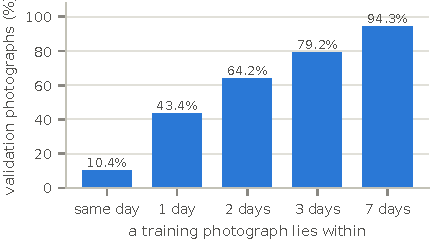
\includegraphics[width=0.62\textwidth]{figures/fig_temporal.pdf}
\caption{Fraction of validation photographs that have a training photograph within a given time
window, for the canonical split (from \file{docs/leaderboard-analysis.md}).
\generatedby{book/make\_book\_figures.py:fig\_temporal}}
\label{fig:val-temporal}
\end{figure}

We cannot fix this by removing training photographs close in time to each validation photograph,
because only 6 of the 106 validation photographs lie more than a week away from every training
photograph. The alternative, implemented in \file{shared/data\_split.py:make\_temporal\_split},
holds out five contiguous blocks of time spread across the years 2011--2022, and discards every
photograph within seven days of a block boundary. In this split no validation photograph has a
training photograph within a week, at the cost of 23 training photographs. Holding out blocks in
this way is the standard remedy for data with temporal or spatial structure~\citep{roberts2017}.

We nevertheless kept the canonical split for our main comparisons, for the following reason. When
we compare two variants of a model on the same split, such as a pipeline with and without erosion,
both variants benefit from the same leak, so their ranking remains valid. What the leak inflates is
the absolute value of the score. For absolute values, the leaderboard remained our reference
throughout the project.

\section{From validation to the leaderboard}\label{sec:val-transfer}
How well does a validation score predict the public score? Figure~\ref{fig:val-public} plots the
\ValPublicPoints{} submissions for which we recorded a validation score. Most of them follow a
simple rule: the public score is between 0.067 and 0.078 lower than the validation score. The
Mask2Former submissions lie at the top of this band or just above it. The deployed model scored
\FloatFortyPQ{} on validation and \BestPublic{} on the leaderboard, an offset of about 0.06.

\begin{figure}[t]
\centering
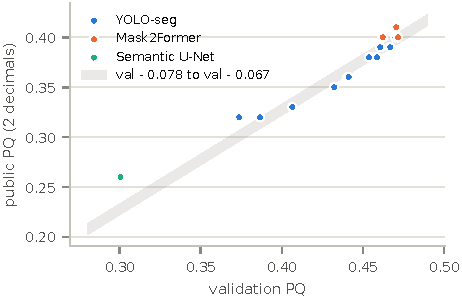
\includegraphics[width=0.66\textwidth]{figures/fig_val_public.pdf}
\caption{Validation PQ against public PQ for every submission whose description records its
validation score. The grey band marks the validation score minus 0.067 to 0.078.
\generatedby{book/make\_book\_figures.py:fig\_val\_public}}
\label{fig:val-public}
\end{figure}

\emph{Changes} in the score transfer less regularly than the scores themselves. The following
three changes had similar effects on validation but quite different effects on the leaderboard:
\begin{center}\small
\begin{tabular}{@{}lccc@{}}
\toprule
change & validation & public & fraction transferred \\
\midrule
inference at 2048 instead of 1280 & $+0.033$ & $+0.010$ & 30\% \\
one-pixel erosion of every mask & $+0.034$ & $+0.030$ & 88\% \\
a mask refiner (a deliberate regression) & $-0.008$ & $-0.010$ & 122\% \\
\bottomrule
\end{tabular}
\end{center}
These percentages must be read with care. Each public difference is the difference of two numbers
rounded to two decimal places, so a displayed change of $+0.010$ is consistent with any true change
between 0 and $+0.02$, and the 30\% in the first row could be anything from 0\% to 60\%. We never
established why the three changes transferred at different rates, and we do not speculate about it
here.

A weaker conclusion held up, and it turned out to be more useful. Every change that moved the
validation score by more than about 0.01 kept its sign on the leaderboard, whereas smaller changes
did not show up reliably. For example, the fine threshold sweep of exp057 scored 0.0028 above the
configuration that we later submitted as exp062, yet the two appeared on the leaderboard as 0.38
and 0.39 respectively. Similarly, exp082 added 77 masks to exp062, gaining 0.0035 on validation,
and appeared as 0.38. We therefore used the validation score as a \keyterm{gate} rather than as a
forecast. A change had to improve the validation score by a margin larger than its noise before it
earned a submission, and we accepted that the leaderboard might then disagree about the size of the
improvement.

The gate has a further limitation: it compares variants of \emph{one} family of models much better
than it compares different families. Our best YOLO ensemble and the deployed Mask2Former differed
by only 0.0024 on validation, yet the leaderboard separated them by 0.02. Conversely, a calibrated
ensemble of the two scored 0.001 higher than the Mask2Former alone on validation, but it appeared as
0.40 on the leaderboard against the Mask2Former's 0.41. When two different architectures tie on
validation, only a submission can separate them.

\subsection{Explanations we checked and rejected}\label{sec:val-rejected}
There are two textbook explanations for a gap between validation and test scores, and we measured
both. The first is that the test data differ from the training data, for example because they come
from other years or stations; in that case models would generalise worse to them. They do not
differ, as Figure~\ref{fig:data-years} shows. The second is a difference in weighting. Our
validation score counts a photograph once per annotator, and a photograph that three experts chose
to label might be easier than average. Reweighting the validation score so that each photograph
counts once changed it by only 0.0008.

What remains is ordinary generalisation error, together with the sampling noise that comes from
scoring half of 180 photographs. We also tested a third possibility with a deliberate probe: that
the test labels might be more inclusive than those of a single annotator, for example because they
were a consensus of several. We submitted a rule (exp028) that admitted many more candidates and
scored 0.041 \emph{worse} on validation. If the test labels had been more inclusive, it would have
scored well on the leaderboard; instead it scored 0.32, which is what the usual offset predicts.

\section{Measuring the ceiling before building}\label{sec:val-oracles}
Perhaps the most useful habit we developed was to ask, before building anything, how much an idea
could be worth at best. An \keyterm{oracle} answers this question by cheating: it uses the ground
truth to make the decision that the proposed method would have to make, and so it measures the best
result that any method of that kind could achieve. An oracle is never a submission; it is an upper
bound that tells us whether the idea is worth pursuing.

A testing manual that we adopted for the project turns this idea into a sequence of three steps,
which we applied most carefully in experiments exp113 to exp118.
\begin{enumerate}[leftmargin=*,itemsep=2pt]
\item \textbf{Ceiling.} Measure the largest gain in PQ that each family of repairs could achieve,
using an oracle. Discard the families whose ceiling is too small to matter.
\item \textbf{Operator.} Give the real repair operator a perfect trigger, which tells it, using the
ground truth, which instances to act on. Measure how much of the ceiling it recovers.
\item \textbf{Gate.} Only then build the real trigger that decides where to act, and measure the
precision it needs to break even.
\end{enumerate}
The order matters. If we reject an idea because its trigger failed, we have learned nothing about
the repair that the trigger was supposed to activate. We made this mistake at one point and later
corrected it, as we describe in Chapter~\ref{ch:post}.

A related discipline is \keyterm{pre-registration}.\footnote{Pre-registration is standard practice
in clinical trials and in experimental psychology, where it guards against choosing the hypothesis
after the data have been seen~\citep{nosek2018}.} Before spending money on a GPU run, we wrote down the hypothesis, the expected gain, and the result that would justify continuing or abandoning
the idea (\file{docs/PREREGISTRATION.md}). We then compared the outcome with numbers that had been
fixed in advance, instead of numbers chosen after seeing the result. The pre-registration written
before the final Mask2Former run, for example, recorded that the architecture had not yet been
tested properly, because the only previous attempt had been stopped long before its training
schedule finished (Section~\ref{sec:train-first}).

\section{Ways to fool ourselves}\label{sec:val-traps}
Each of the following errors occurred during the project, and each produced a validation number
that looked meaningful but was not.

\paragraph{Selecting on the validation set.} If we choose the best of eight configurations, or the
best of ten checkpoints, on the validation split, the score of the winner is optimistic, because
part of its advantage is luck. The deployed Mask2Former checkpoint was chosen in this way, and our
technical report says so. In another case (exp126) we observed a gain of 0.0028 that rested on four
predictions crossing the matching threshold, in the best of eight settings; we recorded it as noise.

\paragraph{Changing the unit of counting.} The validation split has 106 photographs but 180 records,
and a count made in one unit cannot be compared with a count made in the other
(Section~\ref{sec:metric-pooling}).

\paragraph{Changing the resolution.} In exp094 we found that scoring the masks of a model that works
on crops at the resolution of the crops, against a baseline scored at the native resolution, raised
the mean IoU by 0.012 with no model involved at all, because nearest-neighbour resampling happens to
round boundaries favourably. IoU should always be measured at the native resolution.

\paragraph{Comparing filtered and unfiltered populations.} SQ is an average over matched pairs only,
so it cannot be compared with a mean IoU computed over all instances
(Section~\ref{sec:metric-sq-properties}).

\paragraph{Quoting a downstream statistic as an upstream fact.} At one point our notes said that 284
missed filaments had ``zero overlap with any prediction''. This described the set of predictions
that remained \emph{after} the confidence threshold had been applied. In the full pool of candidate
masks, only 65 of those filaments had never been proposed at all
(Section~\ref{sec:recall-stages}).

\paragraph{Deploying something other than what was validated.} We once validated a fusion rule
with its second model run at a confidence floor of 0.05, and then prepared it for deployment with
that model run at a floor of 0.30. The deployed rule would have removed 312 candidates instead of a
handful. We caught the mistake because the deployment file had 979 rows, whereas the validated rule
predicted about 1,229.

The defence against the last error became a standard part of our pipeline. Every deployment path
replays its rule on the validation split, checks that it reproduces the validated score to within a
small tolerance, and checks a cheap invariant such as the number of rows before it writes a single
test prediction (Section~\ref{sec:sub-replay}).

\section*{Exercises}
\begin{exercise}{Leakage through records}
Split the records at random, holding out 15\%. How many validation records share their photograph
with a training record? Using the numbers of records per photograph from
Section~\ref{sec:data-magfilo}, estimate how strongly this leak could inflate a validation score.
\end{exercise}

\begin{exercise}{Temporal neighbours}
For each validation photograph, compute the time to the nearest training photograph, and reproduce
Figure~\ref{fig:val-temporal}. Then do the same for the temporal split in
\file{shared/data\_split.py}.
\end{exercise}

\begin{exercise}{Two decimal places}
Suppose that the public PQ equals the validation PQ minus 0.072, plus Gaussian noise with a standard
deviation of 0.01. Which validation score gives a 50\% chance of the leaderboard displaying 0.41?
Which gives a 90\% chance? How many submissions would you need to distinguish an
improvement of 0.005 from noise?
\end{exercise}

\begin{exercise}{An oracle}
Write an oracle that removes every false positive from the deployed model's validation predictions,
and compute the resulting PQ. Using Section~\ref{sec:metric-agreement}, explain why no real method
can reach it.
\end{exercise}
